\subsection{Cam-Clay plasticity}
\label{subsec:Mp3}

\subsubsection{Definition}
\label{subsubsec:Mp3_def}

This axisymmetric benchmark is usually discussed to verify a critical state plastic mode, e.\,g., the Cam-Clay model. 

\subsubsection{Solution}
\label{subsubsec:Mp3_sol}

For the finite element solution, a quarter of a cylindrical specimen is considered with a diemater of $5\,$cm and a length of $10\,$cm. The bottom surface is roller supported, and a vertical (axial) displacement is prescribed at the top surface until the specimen is compressed at 50\,\% of the initial length. Displacements of the top surface in radial direction are allowed. The lateral surface of the cylinder is free of tractions. The material parameters are summarized in Table~\ref{Mp_tab:m_cc_s}.

\begin{table}[!htb]
\centering
\caption{Material parameters}
\label{Mp_tab:m_cc_s}
\begin{tabular}{llll}
\toprule
Symbol & Parameter & Value & Unit \\
\midrule
$\nu$       & Poisson's ratio                   & $\ \,0.30$ & -- \\
$M$         & Slope of critical state line      & $\ \,1.20$ & -- \\
$\lambda_c$ & Virgin compression index          & $\ \,0.20$ & -- \\
$\kappa_c$  & Swelling\,/\,recompression index  & $\ \,0.02$ & -- \\
${p_s}_{cn0}$ & Initial preconsolidation pressure & $60.00$    & -- \\
$e_0$       & Initial void ratio                & $\ \,1.50$ & -- \\
\bottomrule
\end{tabular}
\end{table}

\begin{minipage}{0.395\textwidth}
\subsubsection{Results}
\label{subsubsec:Mp3_res}

The relationship between von~Mises type stress, the second stress invariant, and the axial strain is illustrated in Fig.~\ref{Mp_fig:m_cc_s_r}. The results agree well with data presented in \cite{SheSloYu00}.
\end{minipage}
\hspace*{0.1\textwidth}
\begin{minipage}{0.49\textwidth}
\begin{figure}[H]
  \begin{center}
    \includegraphics[scale=0.3]{PART_II/M/cc_s_s_e.eps}
  \end{center}
  \caption{Axial strain vs. von Mises type stress }
  \label{Mp_fig:m_cc_s_r}
\end{figure}
\end{minipage}


